\section{Transformación de Gauss}
El sistema que se presentará a continuación (extraído de \cite{Viana}) está relacionado con otro importante algoritmo en Teoría de números, que es la expansión de un número en fracción continua cuyo origen se remonta al problema de hallar la mejor aproximación racional para un número real cualquiera. Vamos a describir ese algoritmo:\\

Dado un número $x \in(0,1),$ sean
\[
a_{1}=\left\lfloor\cfrac{1}{x}\right\rfloor \quad y \quad T_{1}=\cfrac{1}{x}-a_{1}
\]
Note que $a_{1}$ es un número natural y $T_{1} \in[0,1)$ entonces se tiene:
\[
x=\cfrac{1}{a_{1}+T_{1}}
\]
Suponiendo que $T_{1}$ $\neq 0$, podemos repetir el proceso , definiendo
\[
a_{2}=\left\lfloor\cfrac{1}{T_{1}}\right\rfloor \quad y \quad T_{2}=\cfrac{1}{T_{1}}-a_{2}
\]
Entonces 
\[
T_{1}=\cfrac{1}{a_{2}+T_{2}} \quad y \quad por \quad tanto \quad x=\cfrac{1}{a_{1}+\cfrac{1}{a_{2}+T_{2}}}
\]
Por recurrencia, para cada $n \geqslant 1$ tal que $T_{n-1} \in(0,1)$ se define
\[
a_{n}=\left\lfloor\cfrac{1}{T_{n-1}}\right\rfloor \quad y \quad T_{n}=\frac{1}{T_{n-1}}-a_{n}
\]
y se tiene: 
\begin{equation}
    x=\cfrac{1}{a_{1}+\cfrac{1}{a_{2}+\cfrac{1}{\ldots+\cfrac{1}{a_{n}+
    T_{n}}}}}
    \label{equa1}
\end{equation}

Se puede mostrar que la sucesión
\begin{equation}
    \alpha_{n} = \cfrac{1}{a_{1}+\cfrac{1}{a_{2}+\cfrac{1}{\ldots+\cfrac{1}{a_{n}}}}}
    \label{equa2}
\end{equation}
converge para $x$ cuando $n\to\infty$ y es usual traducir este hecho escribiendo
\begin{equation}
    x=\cfrac{1}{a_{1}+\cfrac{1}{a_{2}+\cfrac{1}{\ldots+\cfrac{1}{a_{n}+\cfrac{1}{\ldots}}}}}
    \label{equa3}
\end{equation}
que es llamada la expansión en fracción continua de $x$.

\begin{obs}
Notemos que la sucesión $\{\alpha_{n}\}_{n}$ definida en (\ref{equa2}) consiste de los números racionales. De hecho, estos son los números racionales que mejor aproximan al número $x$, en el sentido de que $\alpha_{n}$ está más próximo de $x$ que de cualquier otro número racional con denominador menor o igual que el denominador de $\alpha_{n}$ (escrito en su forma irreducible.)
Es decir,
$$
\alpha_{n}=[a_{1},a_{2},a_{3},\ldots,a_{n}]=\cfrac{p_{n}}{q_{n}}
$$
Sea $x=[a_{1},a_{2},a_{3},\ldots]$ una fracción continua infinita. Por la definión de aproximación diofántica $k\geq1$ y $1<q_{n}<k$ entonces:
$$
0<\left|x-\cfrac{p_{n}}{q_{n}}\right|<\frac{1}{kq_{n}}
$$
\end{obs}

\begin{obs}
Observemos también que para obtener (\ref{equa3}) suponemos que $T_{n}\in (0,1)$ para todo $n\in\mathbb{N}.$ Si encontramos algún $T_{n}=0$, el proceso para en ese momento y consideramos (\ref{equa1}) la expansión en franción continua de x. Claro que esto último caso ocurre solamente si x es un número racional.
\end{obs}

Ahora, el algoritmo de expansión en fracción continua esta conectado con el sistema dinámico en el intervalo [0,1) que vamos definir a continuación.

\begin{defi}
La Transformación de Gauss es definida por

\[
T:[0,1) \rightarrow[0,1)\quad,\quad T(x)=\left\{\begin{array}{c}
\cfrac{1}{x}-\left\lfloor\cfrac{1}{x}\right\rfloor, \text{ si x } \neq 0  \\\\
0, \text{ si x }  = 0
\end{array}\right.
\]
Definimos $T^{0}(x)=x$ e inductivamente $T^{i+1}(x)=T(T^{i}(x))$.
\end{defi}

\begin{obs}
Un número $x\in (0,1)$ es irracional si y solamente si $T(x)$ es irracional. Por tanto, un número $x$ es irracional si y solamente si, $T^{n}(x)$ es irracional (luego no nulo) para todo $n\geq0.$
\label{obs2}
\end{obs}

Además, el gráfico de $T$ puede ser esbozado fácilmente, a partir de la siguiente observación:
\begin{obs}
Para todo $x$ en cada intervalo $I_{k}=\left(\frac{1}{k+1},\frac{1}{k}\right]$, $k\geq1$, consideramos la parte entera de 1/x igual a k, por tanto, T(x)=1/x - k. Ver la Figura \ref{fig1}.
\end{obs}
\begin{figure}[h]
    \centering
    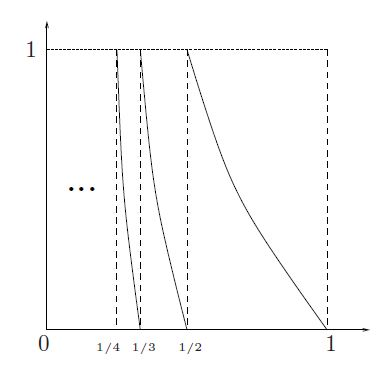
\includegraphics[width=10cm]{chapter1/TG.JPG}
    \caption{Gráfica de la Transformación de Gauss.}
    \label{fig1}
\end{figure}

\break

\begin{ejem}
\textbf{(Expansión de $\sqrt{3}$)} Probemos que $1+[1,2,1,2,\ldots]$ es la expansión en fracción continua de $\sqrt{3}$. Es decir, los cocientes de $\sqrt{3}$ forman una sucesión periódica, donde
$$
a_{2i+1}(\sqrt{3})=1 \quad y \quad a_{2i+2}(\sqrt{3})=2,
$$
para todo $i\geq0$.
Considerando $a_{0}(\sqrt{3})=\lfloor\sqrt{3}\rfloor=1.
$

\end{ejem}
\begin{proof}
Tenemos $a_{0}=\lfloor\sqrt{3}\rfloor=1$ y aplicamos la transformación de Gauss a $y = \sqrt{3}-1 \in (0,1)$,
$$
a_{1}(y)=\left\lfloor\frac{1}{y}\right\rfloor=\left\lfloor\frac{1}{\sqrt{3}-1}\right\rfloor=\left\lfloor\frac{\sqrt{3}+1}{(\sqrt{3}-1)(\sqrt{3}+1)}\right\rfloor=\left\lfloor\frac{\sqrt{3}+1}{2}\right\rfloor=1.
$$
Para calcular $a_{2}(y)$,
$$
a_{2}(y)=\left\lfloor\frac{1}{T(y)}\right\rfloor=\left\lfloor\frac{1}{\frac{1}{y}-\left\lfloor\frac{1}{y}\right\rfloor}\right\rfloor=\left\lfloor\frac{1}{\frac{\sqrt{3}+1}{2}-1}\right\rfloor=
$$
$$
=\left\lfloor\frac{2}{\sqrt{3}-1}\right\rfloor=\left\lfloor\frac{2(\sqrt{3}+1)}{2}\right\rfloor=\left\lfloor\sqrt{3}+1\right\rfloor=2.
$$
Para calcular $a_{3}(y)$,
$$
a_{3}(y)=\left\lfloor\frac{1}{T^{2}(y)}\right\rfloor=\left\lfloor\frac{1}{\frac{1}{T(y)}-\left\lfloor\frac{1}{T(y)}\right\rfloor}\right\rfloor=\left\lfloor\frac{1}{\sqrt{3}+1-2}\right\rfloor=
$$
$$
=\left\lfloor\frac{1}{\sqrt{3}-1}\right\rfloor=\left\lfloor\frac{\sqrt{3}+1}{2}\right\rfloor=1.
$$
Observemos que el proceso de calcular los cocientes $a_{i}(y)$ es el mismo que el de determinar las imágenes de $T^{i}(y)$. En el cálculo anterior obtuvimos
$$
\frac{1}{y}=\frac{1}{T^{0}(y)}=\frac{\sqrt{3}+1}{2}\quad,\quad \frac{1}{T^{1}(y)}=\sqrt{3}+1.
$$
Por inducción tendríamos que:
$$
\frac{1}{T^{2i}(y)}=\frac{\sqrt{3}+1}{2}\quad,\quad\frac{1}{T^{2i+1}(y)}=\sqrt{3}+1.
$$
Entonces para los $a_{i}$ tendríamos
$$
a_{2i+1}(y)=\left\lfloor\frac{1}{T^{2i}(y)}\right\rfloor = \left\lfloor\frac{\sqrt{3}+1}{2}\right\rfloor=1,
$$
$$
a_{2i+2}(y)=\left\lfloor\frac{1}{T^{2i+1}(y)}\right\rfloor = \left\lfloor\frac{\sqrt{3}+1}{2}\right\rfloor=2
$$
Entonces $y=\sqrt{3}-1=[a_{1},a_{2},a_{3},\ldots]$, entonces $\sqrt{3}=1+[a_{1},a_{2},a_{3},\ldots]$. Por tanto, la expansión en fracciones continuas de $\sqrt{3}$ es dada por $1+[1,2,1,2,\ldots]$.
\end{proof}

Continuando con el estudio de las expansiones en fracción continua de un número real (el caso interesante es el caso de los número irracionales). Hemos visto que a cada número irracional $x$ le asociamos usando la transformación de Gauss, su sucesión infinita $\{a_{k}\}_{k\geq0}$ de cocientes. 
\\

Donde un resultado importante será el siguiente Teorema que afirma que la sucesión de cocientes de un número irracional es infinita y que toda sucesión infinita de números naturales es la sucesión de los cocientes de un único número irracional. Obtenemos así una correspondencia biunívoca entre los números irracionales y las sucesiones infinitas de los números naturales.
\\

Formularemos de forma precisa estos resultados. Denotando por $\Sigma_{\infty}$ el conjunto de las sucesiones infinitas de los números naturales, $j=\{j_{k}\}_{k\in\mathbb{N}}$, $j_{k}\in\mathbb{N}$ y por $\mathbb{I}_{(0,1)}$ el conjunto de los números irracionales del intervalo (0,1). Considere la transformación
$$
\mathfrak{G}:\mathbb{I}_{(0,1)}\longrightarrow\Sigma_{\infty} \quad,\quad \mathfrak{G}(x)=\{a_{k}(x)\}_{k}
$$
que asocia a cada número irracional $x$ con su sucesión de cocientes.

\begin{teo}
La función $\mathfrak{G}$ es una biyección.
\label{teo3-1}
\end{teo}

\begin{proof}\hfill
\begin{itemize}
    \item[]Afirmación 1.$\mathfrak{G}$ es inyectiva. \\
    En efecto, sean $x,y\in\mathbb{I}_{(0,1)}$ y supongamos $\mathfrak{G}(x)=\mathfrak{G}(y)$ entonces  $a_{n}(x)=a_{n}(y)$ para todo $n\in\mathbb{N}$ entonces, tendriamos que $$
    x=\displaystyle\lim_{n\to\infty}[a_{1}(x),\ldots,a_{n}(x)]=\displaystyle\lim_{n\to\infty}[a_{1}(y),\ldots,a_{n}(y)]=y
    $$
    Entonces $x=y$.
    \item[]Afirmación 2. $\mathfrak{G}$ es sobreyectiva.
    \\
    En efecto, consideramos cualquier sucesión de números naturales $\{a_{n}\}_{n\in\mathbb{N}}$. Existe $x\in\mathbb{I}_{(0,1)}$ y como todo número real se puede expresar como fracción continua, tenemos que $x=[a_{1},\ldots,a_{n},\ldots]$\\
    Ahora, como la expresión en fracción continua de un número irracional es único $$[a_{1},\ldots,a_{n},\ldots]=x=[a_{1}(x),\ldots,a_{n}(x),\ldots].$$
    entonces $a_{n}=a_{n}(x)$ para todo $n\in\mathbb{N}$  y por tanto $\mathfrak{G}(x)=\{a_{n}\}_{n\in\mathbb{N}}$
\end{itemize} 
\end{proof}

Tenemos que el teorema anterior establece una relación biunívoca entre los números irracionales $\mathbb{I}_{(0,1)}$ del intervalo (0,1) y las sucesiones infinitas de los números naturales $\mathbb{N}^{\mathbb{N}}$: $x\mapsto[a_{1}(x),\ldots,a_{k}(x),\ldots]$. Lo cual significa que los números irracionales se caracterizan por tener expansión en fracciones continuas infinitas. En el siguiente capítulo obtendremos un interesante resultado: un número irracional tiene expansión periódica (puramente periódica o periódica a partir de un determinado término) si y solamente si es solución de una ecuación algebraica de segundo grado. Un ejemplo de este tipo de número es el número aúreo que es una raíz de la ecuación $x^{2}-x-1=0$.
\newpage
